\documentclass[12pt, titlepage]{article}
\usepackage[utf8]{inputenc}
\usepackage{float}
\usepackage[ngerman]{babel}
\usepackage[stable]{footmisc}
\usepackage{graphicx}
\usepackage[a4paper,lmargin={2cm},rmargin={2cm},
tmargin={2.5cm},bmargin = {2.5cm}]{geometry}
\usepackage{caption}

\usepackage{adjustbox}
\let\oldhash\#%
\DeclareRobustCommand{\#}{\adjustbox{valign=B,totalheight=.57\baselineskip}{\oldhash}}%

\usepackage{hyperref}
\hypersetup{
    colorlinks,
    citecolor=black,
    filecolor=black,
    linkcolor=black,
    urlcolor=blue
}

\usepackage{color}
\definecolor{codegreen}{rgb}{0,0.6,0}
\definecolor{codegray}{rgb}{0.5,0.5,0.5}
\definecolor{codepurple}{rgb}{0.58,0,0.82}
\definecolor{backcolour}{rgb}{0.95,0.95,0.92}

\usepackage{listings}
\lstset{literate=%
  {Ö}{{\"O}}1
  {Ä}{{\"A}}1
  {Ü}{{\"U}}1
  {ß}{{\ss}}1
  {ü}{{\"u}}1
  {ä}{{\"a}}1
  {ö}{{\"o}}1
}
\lstdefinestyle{code}{
    backgroundcolor=\color{backcolour},   
    commentstyle=\color{codegreen},
    keywordstyle=\color{magenta},
    numberstyle=\tiny\color{codegray},
    stringstyle=\color{codepurple},
    basicstyle=\ttfamily\footnotesize,
    breakatwhitespace=false,         
    breaklines=true,
    lineskip=2pt,                
    captionpos=b,                    
    keepspaces=true,
    language=[Sharp]C,
    morekeywords={int2},
    numbers=left,                    
    numbersep=5pt,                  
    showspaces=false,                
    showstringspaces=false,
    showtabs=false,                  
    tabsize=2,
    inputencoding=utf8
}

\linespread{1.25}

%Variablen
\newcommand{\myTitle}{Steigerung der Performanz in Videospielen durch Datenorientierte Programmierung}

\begin{document}
\begin{titlepage}
\centering
{\huge Friedrich-Schiller-Universität Jena \par}
{\large Fakultät für Mathematik und Informatik\par}
\vspace{1.5cm}
{\huge\bfseries \myTitle\par}
\vspace{2cm}
{\Large Bachelorarbeit zur Erlangung des akademischen Grades\\Bachelor of Science (B.Sc.) \par}
\vspace{3cm}
{\large vorgelegt von Dennis Untiet\\Matrikelnummer: 192151\par}
\vspace{0.5cm}
{\large geboren am 01.10.2001\quad in Esslingen\par}
\vspace{2cm}
{\large Erstgutachter:\\Zweitgutachter:\par} 
\vfill
{\Large Jena, \today}
\end{titlepage}
\newpage 
\thispagestyle{empty}
\quad
\newpage
\thispagestyle{empty}
\section*{Zusammenfassung}
In der Bachelorarbeit über {\myTitle} geht es um Daten-orientierte Programmierung. Insbesondere wird das Entity Component System von Unity betrachtet.
\newpage
\thispagestyle{empty}
\quad
\newpage
\tableofcontents
\newpage 
\thispagestyle{empty}
\quad
\newpage
\section{Einleitung}
Warum Unity?
\newpage
\section{Datenorientierte Programmierung}
\subsection{Was ist das Datenorientierte Design?}
Data-Oriented Design \cite{Data-OrientedDesign}\\
Probleme mit OOP: Hauptspeicher Zugriff und Cache misses. Versuche Code zu Parallelisieren sind zu viel Aufwand und bringen kaum etwas. Code ist sehr komplex.\\Datenorientiertes Design ist ein anderer Ansatz, der diese Probleme zu lösen versucht. Datenorientierung ändert die Sichtweise des Programmierens: Weg von Objekten, hin zu den eigentlichen Daten, wie diese im Speicher liegen und wie sie gelesen und verändert werden. Beim Programmieren geht es immer um das Verändern von Daten. Es ist die Beschreibung wie aus eingegebenen Daten veränderte Daten werden. Daher ergibt es Sinn sich direkt mit den Daten zu befassen. Zusätzlich: \glqq data-oriented design\grqq{}  hat nichts mit \glqq data-driven\grqq{} zu tun.\\ Ideale Daten:\\Kommt auf die Daten an und wie sie genutzt werden. Am besten wenn man die Daten mit möglichst geringem Aufwand nutzen kann. Also kleinstmögliche Veränderung. Das Programms wird um die ideale Datenstruktur gebaut.\\Objekte sind oft wie Bäume gebaut. Objekte interagieren oft mit anderen Objekte \glqq unter\grqq{} ihnen. Iteriert man über eine Anzahl an Objekten passiert das mehrfach mit beliebigen Objekten. Für ein Ideales Layout sollte ein Objekt in Komponenten zerlegt werden. Komponenten der gleichen Art können dann als Gruppe zusammen im Speicher liegen, egal von welchem Objekt sie kommen. Daraus resultierten große Gruppe homogener Daten, welche dann sequenziell verarbeitet werden können.\\Vorteile:\\Parallelisierung: Die Daten können sehr leicht auf mehrere Threads aufgeteilt werden ohne großen Aufwand\\Cache Affinität: Sehr Effizient, da der selbe Code immer wieder ausgeführt wird. Wenn die Daten sequenziell verarbeitet werden resultiert das in sehr guter Performance und fast perfekter Cache Nutzung.\\Modularität: Wenn Code zur Verbesserung der Performance angepasst wird, resultiert das oft in schlechter lesbarem und schlechter wartbarem Code. Bei Konzentration auf die Transformierung der Daten hat man am Ende kleinere Funktionen mit weniger Abhängigkeiten.\\Testing: Unit Test für Objektinteraktionen können kompliziert sein. Im Datenorientierten Design sind Unit Tests jedoch sehr einfach. Eingabe Daten erstellen, Funktion aufrufen und die Ausgabedaten verifizieren.\\Nachteile: Nicht die Lösung für alles. Schwierig zu lernen, da es ganz anders ist. Auch schwierig mit bestehendem prozedurale / Objektorientiertem Code zu verbinden.\\Anwendung: Klassifizierung, wie Daten genutzt werden: read-only / read-write / write-only. Welche Daten werden von dem System gebraucht? Nicht wie verhält sich ein Gegner sonder eher wie sich alle verhalten.\\Platz für OOP?: Teils / teils. Für einzelne Objekte (beispielsweise GUI) kann es sinnvoll sein. Sollte aber dennoch Datenorientiert geschrieben werden.
\\ DOD \cite{DOD}\\
Datenorientiertes Design kann auch mit anderen Programmier Paradigmen co-existieren. Datenorientierung wird mehr gebraucht, da Spiele immer komplexer werden und die Abstraktion durch OOP das Bottleneck sein wird. Überall sind Daten: Graphik auf dem Bildschirm, Positionen und Bewegung von Partikeln und so weiter. All diese Daten müssen auf etwas laufen, sei es eine VM oder etwas konkretes wie der CPU oder der GPU. Diese Daten existieren auf der Hardware irgendwo. Datenorientiertes Design ist das designen von Software, welche Transformationen auf wohldefinierten Daten ausführt. \\
Ein einfaches Beispiel:\\Angenommen man hat im Objektorientierten Personen Objekte, welche Attribute haben, wie Alter, Beruf und Geschlecht. Dann würden diese Daten im datenorientierten beispielsweise in einer Liste gespeichert werden. Wenn man jetzt das Durchschnittsalter von allen vorhandenen Personen errechnen will muss man im Objektorientierten alle Objekte einzeln ansprechen und dort das Alter abfragen und diese dann verrechnen. Im datenorientierten kann man sich aber direkt die Liste von allen Personen hernehmen. Somit ist der Zugriff und die Berechnung des Durchschnittsalter wesentlicher schneller.
\subsection{Umsetzung Datenorientierter Programmierung}
\newpage
\section{Unity's Datenorientierter Technologie-Stack\footnote{https://unity.com/de/dots}}
Die Arbeit basiert auf der Entities Version 1.0.0-pre.65. Dies ist Stand dem 01.04.2023 die aktuellste Version von Unity's \textit{Enitity Component System.}. Da die Version noch nicht final fertiggestellt wurde und noch stark bei Unity in Arbeit ist, kann sich mit der Zeit viel an der Art und Weise, wie Unity Datenorientierte Programmierung umsetzt, ändern. Das Grundkonzept der Datenorientierung Programmierung ist allerdings mit dem Datenorientierten Technologie-Stack festgeschrieben.\\
Unity's Datenorientierter Ansatz wird durch Unity's Datenorientierter Technologie-Stack umgesetzt. Dieser besteht aus drei Teilen:\\
1. Das \textit{Entity Component System} (ECS) für Unity. Dies ist ein Daten-orientierter Framework für Unity. Dieser ist auch kompatibel mit GameObjects, was Unity's üblicher Objektorientierter Ansatz ist.\\
2. Der \textit{Burst Compiler}. Der Burst Compiler übersetzt von IL/.NET Bytecode zu optimierten nativen Code. Es nutzt die LLVM Compiler Infrastruktur.\\
3. Das C\# Job System. Das Job System von Unity erlaubt es parallelen Code zu schreiben, welcher sicher und schnell läuft.\\
Diese drei Teile werden in den folgenden Katpiteln \ref{ecs}, \ref{burst} und \ref{jobs} erklärt
\subsection{Objektorientierte Programmierung in Unity}
Bevor das \textit{Entity Component System} betrachtet wird ein kleiner Exkurs zu der herkömmlichen Weise, wie in Unity gearbeitet wird. Dies ist hilfreich um folgende Kapitel besser zu verstehen. In Unity basiert alles auf \textit{GameObjects}, die das Objektorientierte schon im Namen haben. Die \textit{GameObjects} werden immer in einer Szene erstellt, wobei es mehrere Szenen in einem Projekt geben kann. Es kann beispielsweise eine Szene für den Startbildschirm geben und eine Szene für das eigentliche Spiel. Alles was man in seiner Szene erstellt ist zunächst ein \textit{GameObject} welches man dann mit Leben füllt. Durch Komponenten die man dem \textit{GameObject} gibt, kann man sie zu Licht, Charakteren, oder Gegenständen werden lassen. Die Komponenten sind allerdings anders als die \textit{Components} aus dem \textit{Entity Component System}. In den folgenden Abschnitten erkennt man hierbei jedoch viele Parallelen zu dieser Arbeitsweise. Die Art wie man Code schreibt ist jedoch sehr unterschiedlich. Zugriffe auf Daten anderer \textit{GameObjects} funktionieren so, dass man erst auf das \textit{GameObject} zugreift und dann darüber auf seine Komponenten. Also ein typische Objektorientierter Ansatz.
\subsection{Das \textit{Entity Component System}} \label{ecs}
\begin{figure}[H]
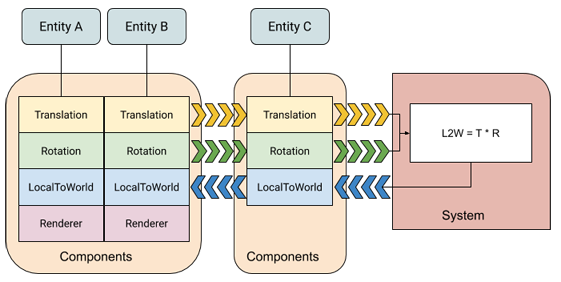
\includegraphics[scale=0.87]{Bilder/ECSConcept.png}
\caption{Zusammenspiel von \textit{Entities}, \textit{Components} und Systemen}
\label{fig:ecs_concept}
\end{figure}
\subsubsection{\textit{Entities}\footnote{https://docs.unity3d.com/Packages/com.unity.entities@1.0/manual/concepts-entities.html}}\textit{Entities} repräsentieren meist Dinge in einem Unity Spiel. Das kann der Spielcharakter, Gegenstände, oder beliebige Gegner sein. Sie können aber auch abstrakte Dinge, wie beispielsweise Events repräsentieren. Ein Entity ist vergleichbar mit einem \textit{GameObject} im Objektorientierten in Unity. \textit{Entities} besitzen hierbei jedoch weder Daten noch ein Verhalten, sondern zeigen lediglich auf, welche Daten beziehungsweise \textit{Components} zueinander gehören. Alle \textit{Entities} in einer Spielwelt gehören zu einer sogenannten Welt\footnote{https://docs.unity3d.com/Packages/com.unity.entities@0.1/manual/world.html}. Zu dieser Welt gehört genau ein \textit{Entitymanager}\footnote{https://docs.unity3d.com/Packages/com.unity.entities@1.0/api/Unity.Entities.EntityManager.html}. Der \textit{Entitymanager} organisiert alle \textit{Entities} in dieser Welt. Mit ihm lassen sich \textit{Entities} erstellen, zerstören, \textit{Components} zu \textit{Entities} hinzufügen, entfernen oder verändern.
\subsubsection{\textit{Components}\footnote{https://docs.unity3d.com/Packages/com.unity.entities@1.0/manual/concepts-components.html}}
\textit{Components} repräsentieren die Daten des Spiels. \textit{Components} speichern die Daten eines \textit{Entity}. Diese Daten werden von Systemen genutzt und verarbeitet. Dabei unterscheidet man zwischen verwalteten \textit{Components} und unverwalteten \textit{Components}. Unverwaltete \textit{Components} werden in Unity als C\# Strukturen implementiert, sind leichtgewichtiger als Klassen. Diese können auch nur unverwaltete Daten speichern. Unverwaltete Daten sind beispielsweise Integer, Boolean, Bytes, Chars, oder andere Strukturen. Verwaltete \textit{Components} werden hingegen als Klassen definiert und können alle Daten halten. Es ist jedoch üblich unverwaltete \textit{Components} zu verwenden, da diese nicht so resourcenintensiv im Speichern und Zugriffen sind. Um ein unverwaltetes Component zu erstellen kann man das IComponentData Interface verwenden. Ein einfaches \textit{Component} könnte also wie folgt aussehen:
\begin{lstlisting}[style=code, caption={Beispiel unverwaltetes \textit{Component}}]
using Unity.Entities;
using Unity.Mathematics;

namespace ECS.Components
{
    public struct ComponentExample : IComponentData
    {
        public int2 position;
        public float speed;
    }
}
\end{lstlisting}
Es gibt aber auch andere Arten von \textit{Components}. Es gibt \textit{Shared components}, \textit{Buffer components} und weitere\footnote{https://docs.unity3d.com/Packages/com.unity.entities@1.0/manual/components-type.html}. Es sind hier nicht alle \textit{Components} relevant, da manche lediglich die Spieleentwickelung mit dem datenorientierten Ansatz erleichtern, aber keine neue Funktion bieten. Zudem gibt es alle Arten von \textit{Components} sowohl als verwaltete als auch unverwaltete \textit{Components}.\\
\textbf{\textit{Shared Components}}: \textit{Shared Components} sind wie der Name schon sagt unter den \textit{Entities} gleich. Sie gruppieren die \textit{Entities} nach dem Wert des \textit{Shared Component}. \textit{Shared Components} werden abseits anderer \textit{Components} gespeichert und sind ein Weg um Datenduplizierung zu vermeiden. Unity speichert zusätzlich alle \textit{Entities}, welche die gleiche Kombination aus \textit{Component} Typen haben und das gleiche \textit{Shared Component} haben, also auch den gleichen Wert, gemeinsam. Dies hat zwar Vorteile, aber auch den großen Nachteil, dass das Ändern von Werten des \textit{Shared Component} ein verschieben der \textit{Entities} im Speicher zufolge hat. Die Probleme hierbei findet man in Kapitel \ref{structuralChanges}. Einen sehr großen und sinnvollen Vorteil haben \textit{Shared Components} in jedem Spiel das mit Unity's ECS entwickelt wird. Das RenderMesh \textit{Component}, also das \textit{Component} welches für das Aussehen der \textit{Entities} zuständig ist, ist immer ein \textit{Shared Component}. Dies ist sinnvoll, da sich diese \textit{Component} sehr selten im Wert ändert und viele \textit{Entities} das selbe RenderMesh \textit{Component} besitzen. Das kann ganz simpel einfach das Aussehen eines Baumes in einem Spiel sein. Oft gibt es viele Bäume in dem Spiel und diese ändern auch ihr Aussehen nicht.\\
\textbf{\textit{Buffer Components}}: Falls man mehrere \textit{Components} der selben Art auf einem \textit{Entity} haben möchte, sind \textit{Buffer Components} sehr hilfreich. Diese agieren wie ein Array von \textit{Components}. Zusätzlich sind \textit{Buffer Components} der Weg um ein Array an Daten zu speichern. Das ist besonder hilfreich, wenn man einem \textit{Entity} ein Inventar geben möchte, da dieses aus mehreren Gegenständen bestehen kann. Also kann man beispielsweise ein \textit{Buffer Component} für ein Inventar so entwerfen:
\begin{lstlisting}[style=code, caption={Buffer \textit{Component} Beispiel}]
using Unity.Entities;

namespace ECS.Components.Other
{
	//Array Kapazität auf acht festlegen
    [InternalBufferCapacity(8)]
    public struct ItemAmount : IBufferElementData
    {
        public int itemID;
        public int amount;
    }
}
\end{lstlisting}
Wie man sieht leitet die Struktur diesmal von IBufferElementData ab, welche den Typ \textit{Buffer Component} angibt. Zusätzlich wird hier das Attribut \textit{InternalBufferCapacity} genutzt. Damit legt man die Kapazität des \textit{Components} fest. Standardmäßig ist die Kapazität die Anzahl an Elementen, welche in 128 Bytes passen. Also hätten wir bei diesem Beispiel eine Kapazität von 16, da in einem \textit{Component} zwei Integer à 32 bit gespeichert werden. Jedoch braucht man für das Inventar beispielsweise nur 8 zu speichernde Gegenstände und kann so den benötigten Speicherplatz reduzieren.
\subsubsection{Systeme\footnote{https://docs.unity3d.com/Packages/com.unity.entities@1.0/manual/concepts-systems.html}}
Systeme beschreiben das Verhalten und beinhalten die Logik zum Transformieren der Daten. Die Systeme laufen ein mal pro ausgegebenem Bild mithilfe der \texttt{OnUpdate} Funktion auf dem \textit{main} Thread. Genau wie bei dem Objektorientierten von Unity gibt es auch hier mehrere Funktionen die zum Start / Ende ausgeführt werden. Zusätzlich kann man noch unter den definierten Systemen eine Reihenfolge festlegen, in der diese ausgeführt werden sollen. So wie bei den \textit{Components} gibt es auch bei den Systemen eine Klasse für verwaltete Daten (welche in diesem Fall von der Klasse SystemBase erbt) und eine Struktur für unverwaltete Daten (welche in diesem Fall das Interface ISystem implementiert). Zusätzlich sind Systeme immer an eine \textit{World} gebunden. Ein System für unverwaltete Daten und ohne implementierte Logik kann folgende Methoden implementieren:
\begin{lstlisting}[style=code, caption={System Beispiel}]
using Unity.Entities;

namespace ECS.Systems
{
    public partial struct ExampleSystem : ISystem, ISystemStartStop
    {
        //Wird beim Erstellen des Systems ausgeführt
        public void OnCreate(ref SystemState state)
        {
        }
        //Wird vor dem ersten OnUpdate des Systems ausgeführt
        public void OnStartRunning(ref SystemState state)
        {
        }
        //Wird für jedes ausgegebene Bild ausgeführt
        public void OnUpdate(ref SystemState state)
        {
        }
        //Wird beim Stoppen des Systems ausgeführt
        public void OnStopRunning(ref SystemState state)
        {
        }
        //Wird beim Zerstören des Systems ausgeführt
        public void OnDestroy(ref SystemState state)
        {
        }
    }
}
\end{lstlisting}
Dabei ist das Interface ISystemStartStop optional und bietet die Möglichkeit bei dem Starten und Stoppen des Systems zusätzlich spezielle Logik auszuführen. Wie man sieht wird allen Funktionen auch eine Referenz des \textit{SystemState} übergeben. Darüber kann man auf verschiedene nützliche Dinge zugreifen, wie beispielsweise die \textit{World}, den \textit{EntityManager}, oder aber auch alle \textit{Components} eines Typs. Eine sinnvolle Herangehensweise ist es, in der \texttt{OnUpdate} Funktion Jobs zu schedulen. Dies wird in Kapitel \ref{jobs} weiter beschrieben.
\subsubsection{Archetypen}
\begin{figure}[H]
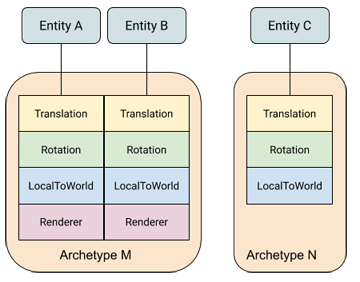
\includegraphics[scale=0.87]{Bilder/ArchetypeConcept.png}
\caption{Konzept von Archetypen}
\label{fig:archetype_concept}
\end{figure}
Ein Archetyp ist eine gewisse Zusammenstellung aus \textit{Components}\footnote{https://docs.unity3d.com/Packages/com.unity.entities@1.0/manual/concepts-archetypes.html}. Jedes \textit{Entity} kann somit einem Archetyp zugeordnet werden. Beispielsweise sind alle \textit{Entities}, welche nur das ExampleComponent haben, einem Archetyp zugeordnet. \textit{Entities} welche zusätzlich \textit{Component} A besitzen gehören zu einem anderen Archetyp. Durch Archetypen ist es möglich, sehr performant, Datenorientiert zu arbeiten. Möchte man in einem System auf verschiedene \textit{Components} Operationen auszuführen, kann man alle Archetypen nach diesen \textit{Components} druchsuchen und muss nicht alle \textit{Entities} durchsuchen. Zusätzlich kann man diese Anfragen an Archetypen cachen um noch mehr Performance zu erreichen. Unity speichert alle \textit{Components} von \textit{Entities} für ein gewissen Archetyp in einem Block. Dieser wird auch \textit{chunk} genannt.
\begin{figure}[H]
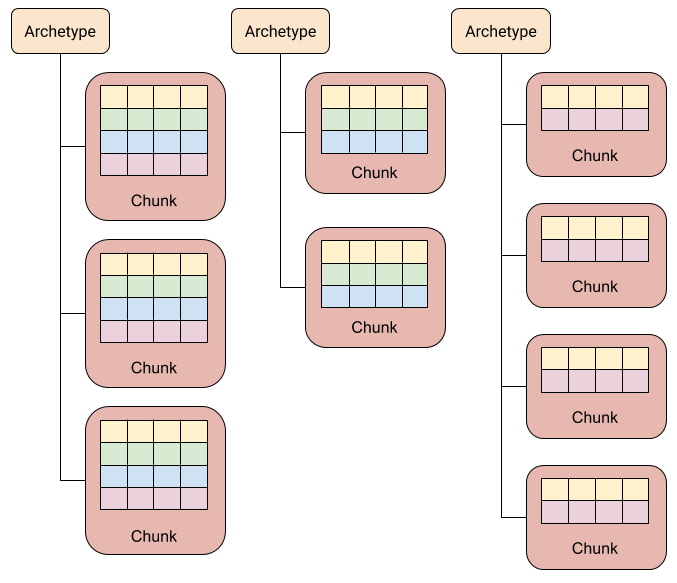
\includegraphics[scale=0.5]{Bilder/ArchetypeChunkDiagram.png}
\caption{\textit{chunks}}
\label{fig:archetyp_chunks}
\end{figure}
Jeder dieser \textit{chunks} ist 16 KiB groß. Demnach hängt es von den \textit{Components} ab, wie viele \textit{Entities} in einen \textit{chunk} passen. Der \textit{chunk} beinhaltet ein Array für jeden Typ der \textit{Components} und zusätzlich ein Array für die \textit{Entity} ID. Pro Arrayindex wird je ein \textit{Entity} gespeichert. Im Index 0 aller Arrays werden die Daten des ersten \textit{Entities} gespeichert. Falls ein \textit{Entity} zerstört, oder in einen anderen \textit{chunk} bewegt wird (falls ein \textit{Component} hinzugefügt, oder entfernt wird), wird das letzte \textit{Entity} an seine Stelle bewegt. Falls ein \textit{chunk} voll ist, erstellt der \textit{EntityManager} einen neuen falls eine \textit{Entity} hinzukommt. Leere \textit{chunks} werden gelöscht.
\subsubsection{Strukturelle Änderungen}\label{structuralChanges}
Strukturelle Änderungen sind eines der wenigen unperformantem Themen in Unity's \textit{ECS}. Strukturelle Änderungen können das Erstellen und Zerstören eines \textit{Entities}, das Hinzufügen und Entfernen von \textit{Components}, oder das Ändern von Daten eines \textit{Shared Components} sein\footnote{https://docs.unity3d.com/Packages/com.unity.entities@1.0/manual/concepts-structural-changes.html}. Also im Grunde alles Operationen, welches das Ändern eines, oder mehrerer \textit{chunks} erfordert. Solche Änderungen könnten andere zur selben Zeit ausgeführten Aktionen invalidieren und müssen deshalb auf dem main Thread ausgeführt werden. Um dennoch Änderungen dynamisch an beliebiger Stelle ausführen zu können, nutzt man den \textit{Entity Command Buffer} (ECB). Mit dem ECB lassen sich strukturelle Änderungen sammeln und zu einem späteren Zeitpunkt in einer festgelegt Reihenfolge ausführen. So lassen sich problemlos aus einem Job strukturelle Änderungen sammeln und nach Beendigung des Jobs, diese auf dem main Thread ausführen. Das kann beispielsweise so aussehen:
\begin{lstlisting}[style=code, caption={ECB Beispiel}]
public void OnUpdate(ref SystemState state)
{
    //Neuer ECB wird erstellt
    EntityCommandBuffer ecb = new EntityCommandBuffer(Allocator.TempJob);
    //Job wird erstellt und der ECB wird übergeben
    new ExampleJob
    {
        ecb = ecb
    //Mit Schedule wird der Job gestartet
    }.Schedule();
    state.CompleteDependency();
    //Strukturelle Änderungen werden abgespielt
    ecb.Playback(state.EntityManager);
    //ECB muss auch wieder disposed werden
    ecb.Dispose();
}
\end{lstlisting}
Also erstellt man einen ECB, reiht verschiedene Aktionen in die Schlange ein und spielt diese auf dem main Thread wieder ab. Danach sollte man den ECB wieder disposen. Das gibt den Speicher für das Objekt wieder frei und räumt gegebenenfalls weitere Ressourcen auf. In dem Job kann man mit dem übergebenen ECB verschiedene Aktionen durchführen. Dies kann beispielsweise so aussehen:
\begin{lstlisting}[style=code, caption={ECB Aktionen Beispiel}]
//Ein Entity erstellen:
Entity newEntity = ecb.Instantiate(e);
//Dem Entity ein Component hinzufügen:
ecb.AddComponent<ExampleComponent>(newEntity);
\end{lstlisting}
Wie ein Job genau aussieht und funktioniert wird in Kapitel \ref{jobs} beschrieben.
\subsection{Burst Compiler} \label{burst}
\subsection{Job System} \label{jobs}
Unity's Job System ist ein guter Weg um parallelen Code zu schreiben.
Run -> Main Thread, Schedule -> ein Helfer Thread, ScheduleParallel -> für jedes mal Execute ein eigener Thread.
\newpage
\section{Factory Spiel in Unity}
Um zu sehen, welches Potential die datenorientierte Programmierung in der Spieleentwicklung bietet wurde eine Spielsimulation sowohl datenorientiert als auch objektorientiert erstellt. Das Spiel, welches simuliert und gemessen wird ist eine Art Aufbauspiel. Verglichen kann es mit dem populären Spiel Factorio\footnote{https://www.factorio.com/}. Hier wird es jedoch etwas schlichter und einfacher gehalten. Um beide Programmierparadigmen miteinander zu vergleichen wird eine kleine Fabrik in die Spielwelt generiert und vervielfältigt. Dies soll den Spieler simulieren. 
\begin{figure}[H]
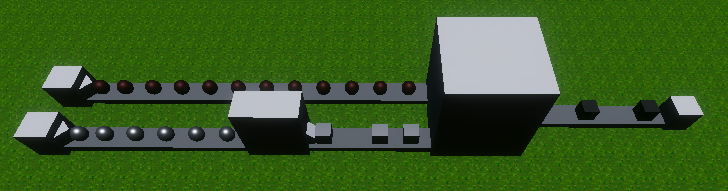
\includegraphics[scale=0.87]{Bilder/Stahl Fabrik.png}
\caption{Eine Stahl Fabrik in der Unity Spielesimulation.}
\label{fig:steel}
\end{figure}
Ganz links befinden sich zwei Kästen. Diese sollen Erzbohrer darstellen welche Eisenerz (silbern) und Kohle (braun) aus der Erde befördern und rechts auf ein Förderband legen. Die beiden Förderbänder transportieren die Kohle und das Eisenerz nach rechts weiter. Das Eisenerz wird als nächstes in Eisenbarren geschmolzen und sind deshalb rechteckig. Die Kohle und die Eisenbarren kommen dann gemeinsam in den großen Würfel, wo sie zu Stahl verarbeitet werden. Dieser Stahl wird dann wieder auf ein Förderband gelegt und in dem kleinen Würfel anschließend gelöscht. Die ganze Produktionskette soll möglichst einem Spiel nahekommen damit es eine möglichst realistische Simulation bietet und die Realität widerspiegelt. Nachfolgend wird gezeigt, wie die Spielsimulation möglichst ähnlich umgesetzt und gebenchmarkt wird.
\subsection{Objektorientierte Programmierung}
In der Objektorientierten Programmierung mit Unity dreht sich alles um GameObjects. Jedes Objekt in der Szene, egal ob sichtbar oder nicht ist ein GameObject. Diese GameObjects können verschiedene Komponenten haben, welche Eigenschaften definieren, also Daten speichern. Diese Komponenten sind jedoch nicht zu verwechseln mit den \textit{Components} aus dem datenorientierten Ansatz von Unity. Diese Komponenten haben jeweils eine \texttt{Start} und eine \texttt{Update} Methode welche das Verhalten definieren. Die Start Methode wird einmalig vor dem ersten Aufruf der \texttt{Update} Methode ausgeführt. Die \texttt{Update} Methode läuft ein mal pro ausgegebenem Bild. Das Skript für das Item sieht wie folgt aus:
\begin{lstlisting}[style=code, caption={Item Komponente OOP}]
using Unity.Mathematics;
using UnityEngine;

public class Item : MonoBehaviour
{
    private int2 pos;
    //Serialisiertes Feld für den Unity Editor
    [SerializeField] private int itemID;

    void Update()
    {
    	//Gegenstand wird zu der übergebenen Position pos bewegt
        transform.position = Vector3.Lerp(transform.position, new Vector3(pos.x, pos.y, -0.5f), Time.deltaTime * 2f);
    }

    public void SetPosition(int2 pos)
    {
        this.pos = pos;
    }

    public int GetItemID()
    {
        return itemID;
    }
}
\end{lstlisting}
Wie man sieht beinhaltet das MonoBehaviour nicht nur die Daten, sondern auch die Logik. Für ein Item benötigen wir zum einen die Position, wohin sich das Item bewegen soll, zum anderen speichern wir auch eine ID über die wir das Item ganz einfach identifizieren können. Das Attribut \glqq SerializeField\grqq{} zwingt Unity dazu ein editierbares Feld im Editor zu erstellen an dem man die itemID setzen kann.
\begin{figure}[H]
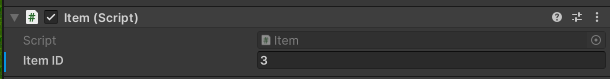
\includegraphics[scale=1]{Bilder/SerializeField.png}
\caption{Ein editierbares Feld in dem Unity Editor. Das Feld wird durch ein public Attribut, oder dem SerializeField Flag erzeugt.}
\label{fig:SerializeField}
\end{figure}
Eine Start Funktion ist in diesem Fall nicht notwendig. Die \texttt{Update} Methode bewegt das Item langsam an die übergebene Position. Time.deltaTime gibt die Zeit in Sekunden von dem letzten Bild bis zu dem momentanen Bild an. Dadurch wird die Bewegung linear.\\Ein weiterer Teil der Simulation ist die Bewegung der Items über das Förderband: 
\begin{lstlisting}[style=code, caption={Förderband Komponente OOP}]
using System.Collections.Generic;
using UnityEngine;

namespace Buildings.Components
{
    public class BeltPath : MonoBehaviour
    {
        private List<ConveyorComponent> beltPath = new ();
        private InputConveyorComponent input;
        private OutputConveyorComponent output;
        private float timeToMove;

        public void Start()
        {
        	//Referenzen auf die Komponenten des GameObjects werden geholt
            input = GetComponent<InputConveyorComponent>();
            output = GetComponent<OutputConveyorComponent>();
            timeToMove = 2f;
        }

        public void Update()
        {
            timeToMove -= Time.deltaTime;
            if(timeToMove > 0) return;
            
            //Gegenstände nach 2 Sekunden bewegen
            var lastBelt = beltPath[^1];
            if (!ReferenceEquals(lastBelt.item, null) && ReferenceEquals(output.GetItem(), null))
            {
            	//Gegenstand von dem letzten Förderbandsegment auf den Output legen
                var item = lastBelt.item;
                var itemComponent = item.GetComponent<Item>();
                itemComponent.SetPosition(output.GetPosition());
                output.SetItem(item);
                lastBelt.item = null;
            }
            //Gegenstände von hinten nach vorne verschieben
            for (int i = beltPath.Count-2; i >= 0; i--)
            {
                var thisConveyor = beltPath[i];
                var lastConveyor = beltPath[i + 1];
                if (!ReferenceEquals(thisConveyor.item, null))
                {
                    if (ReferenceEquals(lastConveyor.item, null))
                    {
                        var item = thisConveyor.item;
                        var itemComponent = item.GetComponent<Item>();
                        lastConveyor.item = item;
                        //Position des Gegenstandes aktualisieren
                        itemComponent.SetPosition(lastConveyor.pos);
                        thisConveyor.item = null;
                    }
                }
            }
            var firstConveyor = beltPath[0];
            //TODO eventuell noch besser machen
            if (!ReferenceEquals(firstConveyor.item, null)) input.SetOccupied(true);
            else input.SetOccupied(false);
            if (!ReferenceEquals(input.GetItem(), null) && ReferenceEquals(firstConveyor.item, null))
            {
                firstConveyor.item = input.GetItem();
                input.RemoveItem();
            }
            timeToMove += 2f;
        }

        public void AddConveyor(ConveyorComponent conveyorComponent)
        {
            beltPath.Add(conveyorComponent);
        }
    }
}
\end{lstlisting}
Für das Förderband wird eine Liste mit vorhandenen Segmenten, der Input, der Output und eine Zeit gespeichert. Die Zeit wird in der Start Methode initialisiert und der Input bzw. Output wird über die Funktion \glqq GetComponent()\grqq{} von dem GameObject geholt. In der \texttt{Update} Funktion wird zunächst nur die timeToMove Variable herunter gezählt. Sollte diese Variable unter Null fallen, werden alle Items von hinten nach vorne ein Segment weiter bewegt sofern dies möglich ist. Ist der Output nicht belegt wird ein vorhandenes Item in den Output gelegt. Items auf den einzelnen Segmenten werden nach weiterbewegt und wenn ein Item im Input liegt wird dies auf das erste Segment weiterbewegt. Immer wenn ein Item weitergegeben wird (egal ob an ein Segment, oder an den Output) wird auch die neue Position an das Item weitergegeben. Durch das bewegen der Items von hinten nach vorne verhindert man, dass sich Items nicht bewegen, obwohl sie es könnten.
\subsection{Datenorientierte Programmierung}
In der datenorientierten Programmierung gehen wir statt der GameObjects auf die Komponenten und Systeme ein. Auch hier zu Beginn die Komponente für ein Item und das dazugehörige System:
\begin{lstlisting}[style=code, caption={Item Komponente ECS}]
using Unity.Entities;
using Unity.Mathematics;

namespace ECS.Components
{
    public struct ItemComponent : IComponentData
    {
        public int2 pos;
        public int itemID;
    }
}
\end{lstlisting}
Auch hier wird die Position und die ID des Items gespeichert. Das dazugehörige System sieht anders aus als das MonoBehaviour im Objektorientierten, die Logik ist jedoch dieselbe:
\begin{lstlisting}[style=code, caption={Item System}]
using ECS.Components;
using Unity.Burst;
using UnityEngine;
using Unity.Entities;
using Unity.Transforms;

[BurstCompile(CompileSynchronously = true)]
public partial struct ItemSystem : ISystem
{
    
    [BurstCompile(CompileSynchronously = true)]
    public void OnUpdate(ref SystemState state)
    {
    	//Job erstellen, Zeit übergeben und schedulen
        new ItemMoveJob
        {
            deltaTime = SystemAPI.Time.DeltaTime
        }.ScheduleParallel();
    }

    [BurstCompile(CompileSynchronously = true)]
    public partial struct ItemMoveJob : IJobEntity
    {
        public float deltaTime;
        
        [BurstCompile(CompileSynchronously = true)]
        private void Execute(ref LocalTransform transform, in ItemComponent item)
        {
        	//Gegenstand wird zu der übergebenen Position pos bewegt
            transform = transform.WithPosition(Vector3.Lerp(transform.Position.xyz, new Vector3(item.pos.x, item.pos.y, -0.5f), deltaTime * 2f));
        }
    }
}
\end{lstlisting}
Jedoch sieht man hier schon Eigenheiten des Entity Component Systems, des Burst Compiler und dem Job System. Das Item System implementiert das Interface ISystem welches für unverwaltete Systeme verwendet werden muss. Zusätzlich ist die Struktur als auch deren Methoden und dem Job mit BurstCompile gekennzeichnet. Diese Kennzeichnung hilft dem Burst Compiler Methoden zu finden, welche mit Burst kompiliert werden sollen. Das Flag CompileSynchronously dient dem testen. Es besagt, dass erst das System durch den Burst Compiler kompiliert werden muss bevor es laufen kann. Andernfalls könnte das System schon laufen, ohne den Burst Compiler genutzt zu haben. Die Methode \texttt{OnUpdate} wird ein mal pro Bild aufgerufen. Sie ist zu vergleichen mit der \texttt{Update} Methode in einem MonoBehaviour. Innerhalb der \texttt{OnUpdate} Methode kommt das Job System von Unity zum Einsatz. Es wird der ItemMoveJob erstellt. Dieser Job funktioniert mit einem LocalTransform Component, welches jedes Entity besitzt und mit dem ItemComponent. Dabei wird das LocalTransform Component zum lesen und schreiben verwendet (erkennbar durch das Keywort ref) und das ItemComponent lediglich zum lesen (erkannbar durch das Keywort in). Auch hier wird nun die Position des Items mithilfe der Lerp Funktion von Vector3 und den Daten im ItemComponent verändert. Dieser Job, welcher die tatsächliche Logik für das Item enthält wird in der \texttt{OnUpdate} Methode parallel gescheduled. Dies ist hier speziell sehr vorteilhaft, da es sehr viele Items auf dem Spielfeld geben kann. Dadurch werden nicht tausende Items nacheinander bewegt, sondern alle zur gleichen Zeit.\\Ein Blick sollte auch auf das Erstellen und Zerstören von Items gelegt werden:
\begin{lstlisting}[style=code, caption={Create Item System}]
using ECS.Components;
using ECS.Components.Other;
using Unity.Burst;
using Unity.Collections;
using Unity.Entities;
using Unity.Mathematics;
using Unity.Transforms;
using UnityEngine;

namespace ECS.Systems
{
    [BurstCompile(CompileSynchronously = true)]
    [UpdateAfter(typeof(ProcessingBuildingSystem))]
    public partial struct CreateItemSystem : ISystem
    {
        private ComponentLookup<InputConveyorComponent> inputLookup;

        [BurstCompile(CompileSynchronously = true)]
        public void OnCreate(ref SystemState state)
        {
        	//Für die OnUpdate Funktion wird das ItemEntitiesComponent gebraucht
            state.RequireForUpdate<ItemEntitiesComponent>();
            inputLookup = state.GetComponentLookup<InputConveyorComponent>();
        }

        [BurstCompile(CompileSynchronously = true)]
        public void OnUpdate(ref SystemState state)
        {
            inputLookup.Update(ref state);
            var ecbSingleton = SystemAPI.GetSingleton<BeginSimulationEntityCommandBufferSystem.Singleton>();
            //Entity Command Buffer wird erstellt
            var ecb = ecbSingleton.CreateCommandBuffer(state.WorldUnmanaged);
            var itemEntities = SystemAPI.GetSingleton<ItemEntitiesComponent>();
            new CreateItemJob
            {
                inputLookup = inputLookup,
                ecb = ecb,
                itemEntities = itemEntities
            }.Schedule();
            state.CompleteDependency();
        }
        
        [BurstCompile(CompileSynchronously = true)]
        [WithNone(typeof(OutputNotFoundTag))]
        public partial struct CreateItemJob : IJobEntity
        {
            public EntityCommandBuffer ecb;
            [ReadOnly] public ComponentLookup<InputConveyorComponent> inputLookup;
            [ReadOnly] public ItemEntitiesComponent itemEntities;

            [BurstCompile(CompileSynchronously = true)]
            private void Execute(ref OutputProcessingBuildingComponent output)
            {
                if(output.itemID == -1) return;
                var itemID = output.itemID;
                var input = inputLookup[output.outputEntity];
                if(input.occupied || input.item != Entity.Null) return;
                output.itemID = -1;
                output.itemCreated = true;
                var itemEntity = itemEntities.GetEntityWithID(itemID);
                var item = ecb.Instantiate(itemEntity);
                ecb.SetComponent(item, LocalTransform.FromPositionRotationScale(new float3(output.pos.x, output.pos.y, -0.5f), quaternion.identity, 0.5f));
                ecb.SetComponent(item, new ItemComponent{pos = output.pos, itemID = itemID});
                ecb.SetComponent(output.outputEntity, new InputConveyorComponent{ item = item, pos = input.pos, occupied = true});
            }
        }
    }
}
\end{lstlisting}
Auch hier sieht man eine Besonderheit des \textit{Entity Component Systems}, der \textit{Entity Command Buffer} (ECB). Dadurch dass strukturelle Änderungen nur auf dem Haupt \textit{Thread} passieren dürfen braucht man einen ECB um diese Änderungen zu sammeln und an späteren Stelle auf dem Haupt \textit{Thread} auszuführem\footnote{https://docs.unity3d.com/Packages/com.unity.entities@1.0/manual/systems-entity-command-buffers.html}. Hier wird der ECB verwendet um strukturelle Änderungen aus einem Job vorzunehmen. Der \textit{Entity Command Buffer} erstellt das Item und ändert noch in den Komponenten die Position des Items.
\newpage
\section{Benchmark}
Auf die Erstellung der einzelnen Spielobjekte ist für den Benchmark nicht relevant. Es werden die Bilder pro Sekunde in Abhängigkeit von der Anzahl der Stahl Fabriken gezählt. 
\newpage
\section{Fazit}
\newpage 
\thispagestyle{empty}
\quad
\newpage
\lstlistoflistings
\newpage
\listoffigures
\newpage
\section{Literaturverzeichnis}
\bibliographystyle{plain}
\bibliography{bibliography}

\newpage
\section{Anlagen}
\newpage
\thispagestyle{empty}
\section*{Selbstständigkeitserklärung}
Ich, Dennis Untiet, erkläre, dass ich die vorliegende Arbeit selbstständig und nur unter Verwendung der
angegebenen Quellen und Hilfsmittel angefertigt habe.\\
Seitens des Verfassers bestehen Einwände die vorliegende Bachelorarbeit für die öffentliche Benutzung im
Universitätsarchiv zur Verfügung zu stellen.\\
Jena, \today, Unterschrift des Verfassenden
\end{document}